\documentclass[10pt,xcolor={dvipsnames}]{beamer}
\usetheme[progressbar=frametitle]{PaloAlto}
\usepackage{appendixnumberbeamer}
\usepackage{booktabs}
\usepackage[scale=2]{ccicons}
\usepackage{pgfplots}
\usepgfplotslibrary{dateplot}
\usepackage[utf8]{inputenc}
\usepackage{fancyvrb}
\usepackage{xspace}
\newcommand\tab[1][1cm]{\hspace*{#1}}
\usepackage{pgf-pie}
\usepackage{color}

\title{Proyecto 1}
\subtitle{Un generador de Scanners}
\date{}
\author{
    José Ceciliano Granados\newline 2016087245
    \newline \newline
    Audra Rodríguez Mora \newline 2015101893
    \newline \newline
    David Valverde Zuñiga \newline 200922986
}
\institute{Instituto Tecnológico de Costa Rica
    \newline Compiladores e Intérpretes
    \newline I Semestre 2019 }
}

\begin{document}

    \maketitle

    \section{Introducción}
        \begin{frame}[fragile]{Introducción}
        \begin{alertblock}{Introducción}
                Flex es una herramienta de análisis lexico desarrollada para la generación de Scanners, programas que reconocen patrones léxicos en el texto.\\
                Su nombre significa "fast lexical analyzer generator" y se encarga de leer las entradas recibidas para generar la descripción de un scanner en forma de pares de expresiones regulares y código C, llamadas "reglas".\\

        \end{alertblock}
        \end{frame}

    \section{Scanning}
        \begin{frame}[fragile]{Scanning}
            \begin{alertblock}{Scanning}
                Mediante proceso de Scanning se identifican los diferentes lexemas de un lenguaje. Flex genera como salida un archivo C que define una rutina en específico, que junto con una biblioteca genera un ejecutable con la capacidad de analizar su entrada para la aparición de expresiones regulares. Cada vez que encuentra una, ejecuta el código C correspondiente.\\
                Todo esto se puede traducir a que Flex es capaz de crear un "Deterministic Finite Automaton" (DFA) que se utilizará para adquirir los diferentes lexemas que se pretenden escánear.
            \end{alertblock}
        \end{frame}


    \section{Gráficos}
        \begin{frame}[fragile,allowframebreaks]{Histograma}
        \begin{alertblock}{Histograma}
            A continuación se presenta un histograma que muestra la cantidad de cada tipo de \textit{token} encontrado en el código fuente:
            \end{alertblock}
        \end{frame}

    \subsection{Gráfico Barras}
        \begin{frame}[fragile]{Histograma} 
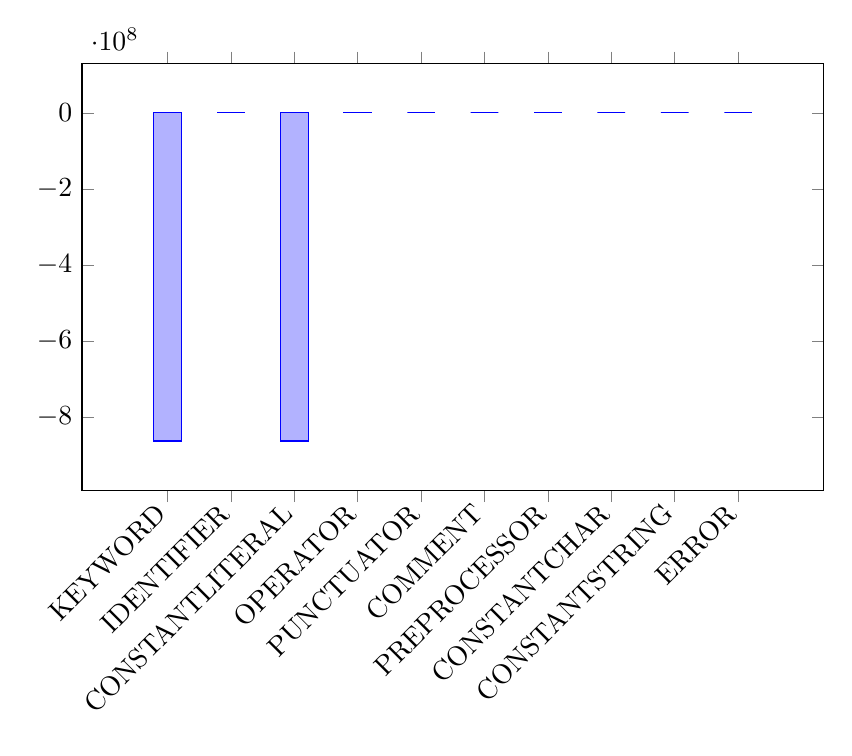
\begin{tikzpicture}     
\begin{axis}[ybar, enlargelimits=0.15, x tick label style={rotate=45, anchor=east},    symbolic x coords={KEYWORD, 
IDENTIFIER, 
CONSTANTLITERAL, 
OPERATOR, 
PUNCTUATOR, 
COMMENT, 
PREPROCESSOR, 
CONSTANTCHAR, 
CONSTANTSTRING, 
ERROR, 
},xtick=data,width=11cm,height=7cm] 
 \addplot coordinates {(KEYWORD,-863060829) 
(IDENTIFIER,32722) 
(CONSTANTLITERAL,-863060830) 
(OPERATOR,32716) 
(PUNCTUATOR,15) 
(COMMENT,0) 
(PREPROCESSOR,0) 
(CONSTANTCHAR,0) 
(CONSTANTSTRING,0) 
(ERROR,0) 
};
\end{axis}  
\end{tikzpicture} 
\end{frame}
    \subsection{Gráfico Pastel}
        \begin{frame}[fragile]{Histograma} 
\begin{tikzpicture} 
\pie[text=legend]{ 0/KEYWORD, 36/IDENTIFIER, 0/CONSTANTLITERAL, 0/OPERATOR, 48/PUNCTUATOR, 0/COMMENT, 1/PREPROCESSOR, 10/CONSTANTCHAR, 0/CONSTANTSTRING, 2/ERROR, }
\end{tikzpicture}
\end{frame}

    \section{Analisis Léxico}
        \begin{frame}[fragile,allowframebreaks]{Analisis Léxico}
        \begin{alertblock}{Codigo fuente}
            A continuación se presenta el código fuente con colores demostrando la división de \textit{tokens}.
            \end{alertblock}
        \end{frame}

        \begin{frame}[fragile,allowframebreaks]{Resaltado de sintaxis}~\color{MidnightBlue}\verb$# 1 "tests/1.c"$\newline\color{MidnightBlue}\verb$# 1 "<built-in>"$\newline\color{MidnightBlue}\verb$# 1 "<command-line>"$\newline\color{MidnightBlue}\verb$# 31 "<command-line>"$\newline\color{MidnightBlue}\verb$# 1 "/usr/include/stdc-predef.h" 1 3 4$\newline\newline\color{MidnightBlue}\verb$# 1 "/usr/include/stdc-predef.h" 3 4$\newline\color{Gray}\begin{verbatim}/* Copyright (C) 1991-2018 Free Software Foundation, Inc.
   This file is part of the GNU C Library.

   The GNU C Library is free software; you can redistribute it and/or
   modify it under the terms of the GNU Lesser General Public
   License as published by the Free Software Foundation; either
   version 2.1 of the License, or (at your option) any later version.

   The GNU C Library is distributed in the hope that it will be useful,
   but WITHOUT ANY WARRANTY; without even the implied warranty of
   MERCHANTABILITY or FITNESS FOR A PARTICULAR PURPOSE.  See the GNU
   Lesser General Public License for more details.

   You should have received a copy of the GNU Lesser General Public
   License along with the GNU C Library; if not, see
   <http://www.gnu.org/licenses/>.  */\end{verbatim}\leavevmode\newline\newline\newline\newline\newline\color{Gray}\begin{verbatim}/* This header is separate from features.h so that the compiler can
   include it implicitly at the start of every compilation.  It must
   not itself include <features.h> or any other header that includes
   <features.h> because the implicit include comes before any feature
   test macros that may be defined in a source file before it first
   explicitly includes a system header.  GCC knows the name of this
   header in order to preinclude it.  */\end{verbatim}\leavevmode\newline\newline\color{Gray}\begin{verbatim}/* glibc's intent is to support the IEC 559 math functionality, real
   and complex.  If the GCC (4.9 and later) predefined macros
   specifying compiler intent are available, use them to determine
   whether the overall intent is to support these features; otherwise,
   presume an older compiler has intent to support these features and
   define these macros by default.  */\end{verbatim}\leavevmode\newline\color{MidnightBlue}\verb$# 52 "/usr/include/stdc-predef.h" 3 4$\newline\color{Gray}\begin{verbatim}/* wchar_t uses Unicode 10.0.0.  Version 10.0 of the Unicode Standard is
   synchronized with ISO/IEC 10646:2017, fifth edition, plus
   the following additions from Amendment 1 to the fifth edition:
   - 56 emoji characters
   - 285 hentaigana
   - 3 additional Zanabazar Square characters */\end{verbatim}\leavevmode\newline\newline\newline\color{Gray}\begin{verbatim}/* We do not support C11 <threads.h>.  */\end{verbatim}\leavevmode\newline\color{MidnightBlue}\verb$# 32 "<command-line>" 2$\newline\color{MidnightBlue}\verb$# 1 "tests/1.c"$\newline\newline\color{MidnightBlue}\verb$# 1 "tests/1.c"$\newline\color{BlueViolet}\verb$main$\color{OliveGreen}\verb$($\color{OliveGreen}\verb$)$ \color{OliveGreen}\verb${$\newline    \color{Sepia}\verb$int$ \color{BlueViolet}\verb$a$\color{OliveGreen}\verb$;$\newline\color{OliveGreen}\verb$}$\newline
\end{frame}



\end{document}
